\section{Background on Native Frameworks}
\label{section:background}

In this section, we provide background on native frameworks using Xamarin as a
concrete example.  Xamarin allows the development of native mobile apps for
multiple platforms while aiming to maximize code-reuse across platforms.
Developers using Xamarin target their apps to its home platform, Windows Phone,
and can re-use much of the same code to build native apps for iOS, Android, and
Mac. In this section, we discuss the structure of a cross-platform app written
using Xamarin, and discuss the techniques that Xamarin uses to allow app logic
and data storage code to be written once and reused across platforms.

A developer using Xamarin can build apps in C\#, using features such as
generics, Linq and the parallel task library. The developer splits the app into
two logical pieces (\figref{figure:appstruct}): \textit{the application core},
which encodes the business logic, and contains code that is common across all
platforms, and \textit{user interface (UI)}, which is written for each platform
and uses the native UI features of that platform, \eg~buttons, widgets, and the
overall look and feel of the specific platform. The developer implements the UI
layer in C\# as well, using native UI design tools such as
\code{Android.Views}, \code{MonoTouch.UIKit} for iOS, and XAML, Silverlight and
Metro APIs for Windows Phone. The functionality and layout of the UI elements
can be controlled by the business logic in the application core, \eg~in
determining which button triggers what functionality in the app.  Xamarin is
built atop the Mono \code{.NET} framework~\cite{mono}, which provides the core
cross-platform implementation of Microsoft's \code{.NET} framework. C\# source
code can be compiled with Xamarin's compiler to produce a native iOS app, or an
Android app with integrated \code{.NET} runtime support. In this case, the C\#
code is compiled to an intermediate language, and packaged with MonoVM
configured for just-in-time compilation on Android.

\begin{figure}[t!]
\centering
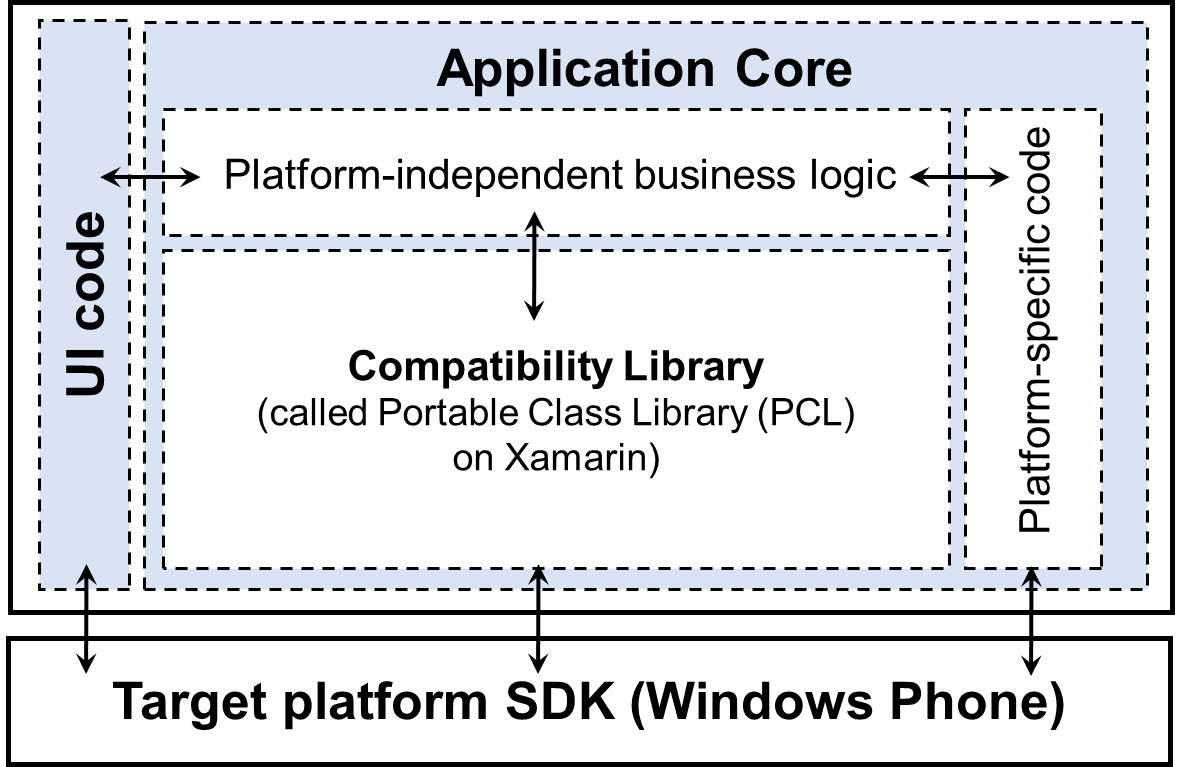
\includegraphics[keepaspectratio=true,width=0.45\textwidth]{figures/appstruct.png}
\mycaption{Structure of a cross-platform app written using Xamarin.}
{\label{figure:appstruct}}
\end{figure}

Xamarin aims to provide support to developers to minimize the amount of
platform-specific code that is needed to port an app across platforms.  To
achieve this goal, one of the main components of the core of a Xamarin-based
app are cross-platform compatibility libraries, also called \textit{portable
class libraries, or PCLs} in Xamarin, a technology originally developed by
Microsoft. On Visual Studio and other Microsoft environments, a PCL is a
special type of a project that allows developers to write code and produce
libraries that can be shared across multiple platforms, such as iOS, Android,
and Windows Phone. To support this, PCLs export an interface of methods and
properties that are portable across platforms, and developers program to this
interface. The app developer encodes platform-independent business logic by
programming to this interface. The PCL provides forwarding stubs that ensures
that calls to methods or property accesses are routed to the correct underlying
platform libraries at runtime.  The developer of the PCL typically identifies
the interface by choosing a set of target platforms that the PCL will support.
Because different platforms provide implementations of differing subsets of the
base \code{.NET} class library, the PCL interface is typically restricted to
the common \code{.NET} functionality that is supported by all the target
platforms. 

PCLs play a key role in Xamarin because they serve as the compatibility layer
between two different platforms. As previously mentioned, about Xamarin's
BugZilla database lists about 7,100 that are related to PCL.  Despite the
functionality provided by the PCLs, some platform-dependent business logic may
be necessary in the application core.  For example, PCLs are still in active
development, and if the app developer wishes to use features that are not
currently supported by the PCL, he has to do so by writing platform-specific
code, called \textit{shared assets} on Xamarin. It is possible to write this
code once and compile it for all desired target platforms using compiler or
pre-processor directives (\eg~code specific to Android or iOS would be guarded
using a directive such as \code{\#ifdef ANDROID} or \code{\#ifdef iOS},
respectively).  Naturally, the goal of projects such as Xamarin is to increase
the coverage provided by their PCLs, so as to minimize the amount of code that
must be written as shared asset projects.

In addition to the application core, the app also includes UI code. Currently,
UI code is largely platform-specific because UI elements, \eg~the look and feel
of buttons and widgets, are customized to specific mobile platforms.
Nevertheless, there are ongoing efforts such as \code{Xamarin.Forms} to even
minimize the amount of platform-specific UI code.

% \todo{How many methods supported in Xamarin's PCLs? What fraction of the .NET
% API still not supported?}

In this paper, we are primarily concerned with testing the functionality of the
PCLs on Xamarin that provide support for platform-independent app code.
Therefore, the test cases generated by \tool\ only target the PCL interface.
Our test cases do not directly target the platform-specific UI code. However,
note that many aspects of the layout and functionality of the UI are controlled
by the business logic, which interacts with the target platform's SDK via the
PCLs.  Therefore, by testing the functionality of the PCLs, we indirectly test
the overall functionality of the app's execution on the target platform
(including its UI).
